\documentclass[type = bachelor, oneside]{whu-thesis}
\usepackage{textcomp,mathcomp}
\usepackage{siunitx}
\usepackage{chemfig}
\usepackage{graphicx}

\whusetup
  {
    info               =
      {
        title          = {金刚石氮-空位色心的\\电荷态调控和性质表征},
        title*         = {Modulation of Charge States and Characterization of Properties\\ in Nitrogen-Vacancy Centers of Diamond},
        student-number = {2020302192129},
        school         = {弘毅学堂},
        author         = {邹迪玮},
        author*        = {Diwei Zou},
        subject        = {学科},
        major          = {微电子科学与工程},
        advisor        = {周利 , 副教授;孙启超 , 研究员},
        direction      = {研究方向},
        date           = {2024/5},
        keywords       = {关键词 1 , 关键词 2 , 关键词 3 , 关键词 4 , 一个非常非常,非常非常长——的关键词 5},
        keywords*      = {key word 1 , key word 2 , key word 3 , key word 4 , {and a very very, very very long key word---the key word 5}},
      },
    style              =
      {
        graphics-path  = {{figures/}{data/}},
        list-of-figures,
        list-of-tables,
      },
    element            =
      {
        innovation     = {pages/innovation},
        abstract       = {pages/abstract},
        abstract*      = {pages/enabstract},
        bibliography   = {ref/refs_all}
      }
  }
\begin{document}

% Chapter 4

\chapter{实验平台的设计与搭建}

\section{共聚焦显微镜光学系统实验平台}
\subsection{共聚焦显微镜的基本原理}
实验室中常见的光学显微镜是通过光源发出自然光(白光)投射到被测样品上,样品的反射或透射光被物镜聚焦到目镜上,通过目镜观察到被测样品的图像。这种显微镜的分辨率受到可见光的波长的限制,通常在0.2 $\mu m$左右。为了提高显微镜的分辨率,人们提出了共聚焦显微镜(Confocal Microscopy)的概念,通过在显微镜中加入共聚焦系统,可以使得显微镜的分辨率提高到0.1 $\mu m$以下。共聚焦显微镜的基本原理是通过激光光源发出的激光束照射到样品上,样品的受到激光的激发后,在退激发的过程中会产生荧光效应释放出光子,被物镜聚焦到探测器上,并将信息传回到电脑。共聚焦显微镜的分辨率受到激光波长和物镜规格的限制,通常能在0.1 $\mu m$以下。共聚焦显微镜的优点是可以观察到样品的表面形貌和内部结构,实现三维的成像,非接触式无损的高分辨率、高灵敏度、高对比度的观察。

对于NV Center而言,由于基态能级结构的电子能被绿光激发,并在退激发的过程中发射声子边带的红光光子,所以共聚焦显微镜的原理可以用于对金刚石中的NV Center进行表征和检测,通过激光的聚焦和荧光的检测,可以实现对不同深度NV Center的三维定位和成像。一般来说,共聚焦显微镜有以下几个主要的部分:激光光源、激光束聚焦系统、样品台、物镜、探测器、数据采集系统等等。平台的构建也有多种方案,通过镜头的放置方式和扫描的运行方式来区分。
\begin{figure}
  \centering
  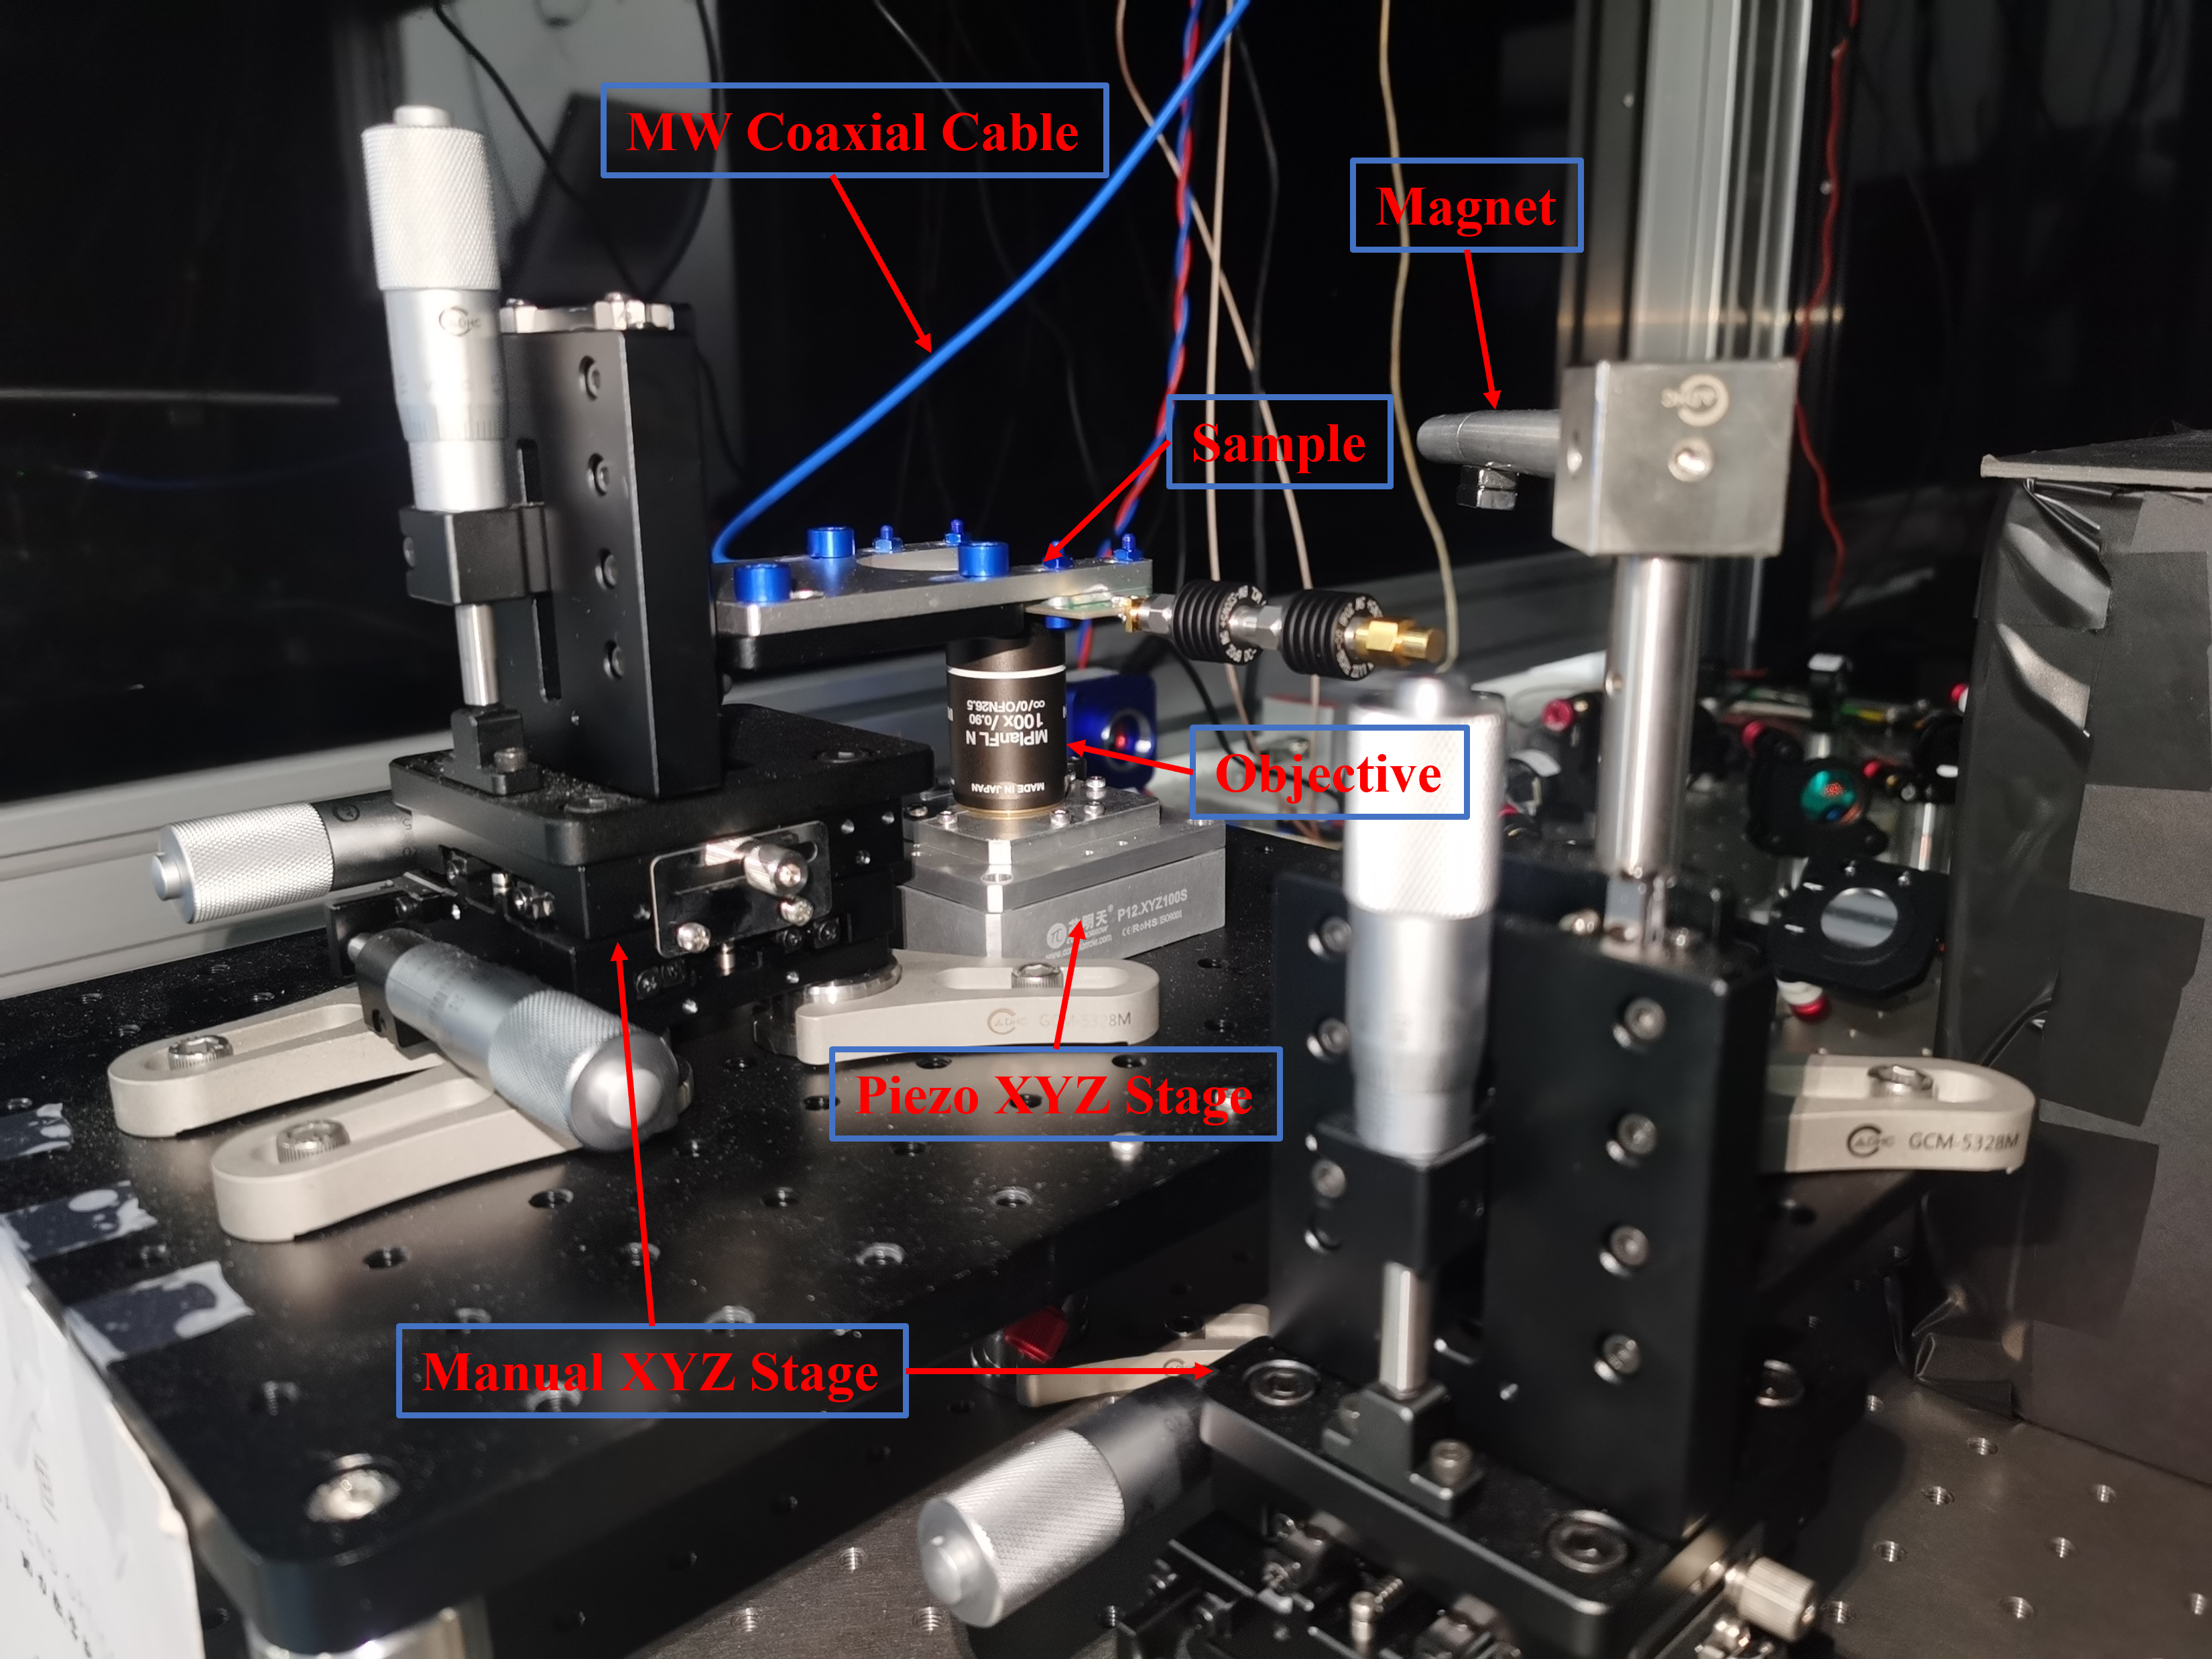
\includegraphics[width=0.8\textwidth]{figures/Chapter 2/Confocal Platform.png}
  \caption[共聚焦显微镜平台]{共聚焦显微镜平台,样品放置于手动XYZ三轴位移台上进行粗调节和聚焦,显微物镜倒置放置于压电纳米XYZ三轴位移台上进行精细扫描和聚焦。微波利用同轴线缆传递到样品表面,磁体也通过三轴手动位移台调节与样品的相对位置。}
  \label{fig: Confocal Platform}
\end{figure}
如图 \ref{fig: Confocal Platform}所示,我们采用的方案是镜头倒置,通过纳米压电位移台移动镜头对样品表面进行扫描的方案。压电位移台为XYZ三轴位移台,移动范围均为100 $\mu m$,精度和稳定性为10 nm的量级,可以实现亚微米级别的扫描和定位。如图 \ref{fig: Confocal Optimizer}所示,展示了Confocal显微镜的Optimize图像,左图为XY方向二维扫描的图像,用于确定NV Center在二维平面的位置;右图为Z方向扫描在不同深度的计数率,用于确定NV Center的深度。我们通过使用的德国Ulm University科研人员开发的基于Python的开源软件Qudi来对整套共聚焦系统进行控制,其中的Optimize功能能够在指定范围内自动寻找计数率高的位置来聚焦寻找NV Center,即图 \ref{fig: Confocal Optimizer}所示效果 \cite{Binder2017}。用于测试的样品的NV Center是通过在Element Six公司生产的电子级金刚石表面注入$^{14}$N离子形成的,所以NV Center的位置大部分在离表面5 $\mu m$内的浅层位置,使其发射的荧光光子能够尽可能多的被物镜所接收,提高实验数据和结果的对比度。
\begin{figure}
  \centering
  \includegraphics[width=0.6\textwidth]{figures/Chapter 2/Confocal Optimizer.png}
  \caption[Confocal显微镜的扫描和Auto Optimize功能]{Confocal显微镜的扫描和Auto Optimize功能。}
  \label{fig: Confocal Optimizer}
\end{figure}

\subsection{共聚焦显微镜的搭建}
如图 \ref{fig: Light Path}展示了实验中的光路简图,其中画出了主要元件,一些用于微调调整光路的普通透镜、反射镜、光阑等原件并未画出。对于532 nm的绿光光路而言,激光器产生的激光在出口处耦合进通过光纤输出,光纤用法兰连接光纤声光调制器(Acousto-Optic Modulator,AOM),经过AOM后在通过光纤输出,并在光纤末端用准直器将激光聚焦为高斯光束。AOM是一种通过压电声学效应改变晶体衍射效应,从而对光信号进行调制的器件。我们使用的AOM的驱动器有模拟和数字两个输入口,通过模拟信号输入不同的电压(0-5 V),可以对光强大小进行无级调节;而利用任意波形发生器(Arbitrary Waveform Generator,AWG)产生高频的高低电平,输入给AOM驱动器的数字接口,则可以实现对激光的快速开关,实现特定序列的脉冲测量,其上升沿和下降沿大约为400 ns。激光输出后,通过一个9:1的消偏振分光棱镜(Non-Polarizing Beam Splitter,NPBS),将透射光和反射光的光强分为9:1的两份,且没有改变偏振方向。经过NPBS后,90 \%的透射光透过NPBS继续在光路中传播,而剩下10 \%的反射光则被光电二极管(Photodioad,PD)收集,将光强成比例地转化为电流通过一个定值电阻,通过测量其两端的电压来实时监测光强的大小。经过NPBS的透射光继续传播,穿过550 nm和600 nm截止波长的两个低通二项色镜(Low Pass Dichroic Mirror,LP DM),通过压电位移台设计的孔洞中进入物镜,聚焦于样品表面。前文中有提到过NV Center会受到532 nm的绿光激发后,退激发的过程中发出637 nm的ZPL和波长更长的PSB,这些荧光被同一个物镜收集并原路返回,这些荧光在遇到600 nm LP DM后被反射向左,经过一个663-800 nm的带通滤波片(Band Pass Filter,BP Filter)后,大部分PSB进入单光子雪崩二极管(Avalanche Photodiode,APD)收集,每次收集到一个光子后就会形成脉冲信号,并将数字信号传递给电脑。
\begin{figure}
  \centering
  \includegraphics[width=1.0\textwidth]{figures/Chapter 2/Light Path.png}
  \caption[共聚焦显微镜光路简图]{共聚焦显微镜光路简图。}
  \label{fig: Light Path}
\end{figure}

对于594 nm的橙光光路而言,大部分的设计与532 nm的绿光光路相似,有一点不同的是这个光路中应用的AOM是空间AOM,激光以空间光的形式,通过一个透镜聚焦进入AOM,在出口处相同位置处放置一个相同焦距的透镜来将光束准直。激光经过空间AOM后,会形成多级衍射光斑,其中一级和负一级衍射光斑是可以通过控制AOM来进行调制的,因此我们利用光阑过滤掉了其他光斑,仅留下了一级衍射光斑在光路中继续传播。由于高斯光束在经过AOM后的形状会变得畸形,所以通过物镜耦合进入光纤传递来进行整形,再通过物镜和五维光纤调整架进行准直。如图 \ref{fig: 594 Collimator}所示,通过调整光纤头的位置,对准物镜的出口,准直的高斯光束会从物镜入口处反向射出。由于594 nm的橙光和532 nm的波长不同,导致相差的微小差异,这套装置实际上相当一个可调焦距的准直镜头,将两束激光聚焦于同一平面内。随后,594 nm的橙光通过550 nm LP DM和532 nm的绿光耦合到一起共轴共线,进入显微物镜从而聚焦于样品表面。
\begin{figure}
  \centering
  \includegraphics[width=1.0\textwidth]{figures/Chapter 2/594 Collimator.jpg}
  \caption[594 nm光纤光束准直]{594 nm光纤光束准直,通过物镜和五维光纤调整架对激光进行准直。}
  \label{fig: 594 Collimator}
\end{figure}

\subsection{金刚石样品}
如图 \ref{fig: Sample}所示,样品被粘在铝合金转接板上,转接板和电路板通过蓝色的铝合金螺丝固定,放置铁磁性材料的磁场干扰,或者再施加磁场的过程中受力而发生位移。电路板两头为SMA射频连接头,一头连接混频器发射的微波信号,另一头连接50 $\Omega$的阻抗衰减。中间贯穿的条带为导线,两侧铺铜接地隔离将电磁场束缚在中心,中间部分焊接一根50 $\mu m$粗的铜线作为微波天线,紧贴样品表面使微波在样品表面辐射。微波源(Microwave Source,MW Source)的信号经过放大器,通过混频器(Mixer)和AWG的信号混合后,通向样品电路板的SMA射频连接头。混合AWG信号的目的是在原有设置的恒定的GHz量级的微波信号基础上,加上一个MHz量级的射频信号,从而实现更精细的Pulsed ODMR测量。图中在混频器后省略了微波开关,其功能是通过AWG控制微波的通断来进行特定的序列测量,比如FID、Rabi Oscillation、Hahn-echo Sequence等。
\begin{figure}
  \centering
  \includegraphics[width=1.0\textwidth]{figures/Chapter 2/Sample.jpg}
  \caption[金刚石样品和微波天线结构]{金刚石样品和微波天线结构。}
  \label{fig: Sample}
\end{figure}

\section{测量过程的设计}
\subsection{数据的采集过程}
在测量的过程中,我们选取了两个序列,分别为连续波序列(Continuous Wave,CW)和脉冲序列(Pulsed)两种形式,CW Measurement的目的是为了检测NV Center的电荷态动态平衡分布情况,而Pulsed Measurement的目的是为了将调控电荷的分布并且将自选转化为电荷态进行表征。在整个过程中,我们需要记录的数据只有时间尺度下的荧光发射光子数。在这个过程中,我们利用了时间标记器(Time Tagger,TT),也就是一种基于Opal Kelly FPGA板卡编程设计和开发的时间数字转换器(Time-to-Digital Converter,TDC),可以记录ns级分辨精度的数字信号数据,用于将左右设备的时序逻辑同步对应。我们将AWG和APD的输出都接入到TT上,通过AWG输出序列来控制TT的计数器触发和记录序列,TT接收到高电平的触发信号后,在设定的记录序列接口处于高电平状态的时候就会持续记录数据。与此同时,将AWG连接控制532 nm绿光和594 nm的橙光AOM驱动器,以及微波开关,由此可以通过AWG控制生成的序列来控制激光快速精准的通断和微波的脉冲。这样我们就可以通过控制AWG的输出信号来实现对NV Center的操控和测量。

在准备阶段,我们可以在启动TT的时候设置每一轮测量的最小时间分辨率和整体的时间尺度,以及与物理接口所对应的信号收集通道、触发接口通道和测量脉冲序列通道。在后续的测量过程中,我们设置的最小时间尺度时间窗口(time bins)的分辨率为10 $\mu s$,每一轮测试为10$^6$个time bins,也就是每一轮序列测试是可以持续采集10 $s$的数据,并将原始数据输出为.npy格式的数组保存。在整个测量过程中,我们需要保证样品表面的温度和湿度保持稳定,以及尽可能的减少外部的振动和磁场干扰,以保证测量的准确性和稳定性。由于受到环境变化的干扰,比如温度、湿度、振动等,已经聚焦好的点位会有轻微的漂移现象,所以我们在会对该点进行定时的重新Optimize。我们设置180轮序列测试为一个循环,在一个循环后序列会自动停止,然后click一次Optimize,重新寻找最佳的聚焦点位,然后再次开始下一个循环,并将所有的180个数据保存到本地文件中。通过设置不同的循环次数,我们能够定制不同的数据累积时间,从而保证不同情况下数据量尽可能地归一性。


\subsection{测量序列的设置和数据的处理}

如图 \ref{fig: Measurement Sequence}所示,(a)图为CW测量序列,(b)图为Pulsed测量序列。
\begin{figure}
  \centering
  \includegraphics[width=1.0\textwidth]{figures/Chapter 2/Measurement Sequence.png}
  \caption[CW和Pulsed测量序列简图]{CW和Pulsed测量序列简图,$t_r$为读出时间窗口,$t_{ini}$为初始化时间长度。}
  \label{fig: Measurement Sequence}
\end{figure}

对于(a)图中CW序列而言,在每一轮10 $s$的测试过程中,594 nm的橙光持续保持开启的状态。由于AOM的开启存在上升沿和稳定性的问题,每次TT计数器的触发接口在开启橙光后10 $\mu s$后,施加一个50 $ns$的高电平脉冲,使计数器启动。随后TT计数器的测量脉冲序列通道保持10 $s$的高电平状态,在这个过程中,TT以10 $\mu s$为时间分辨率窗口进行持续地记录数据。序列结束的时候,保持橙光持续开启2 $\mu s$,以确保测量序列末端的光强稳定。因为是连续测量,所以在设置不同的读出时间$t_r$的时候,只需要通过不同数量的相邻time bins进行合并,即可得到不同的$t_r$,即$t_r = n_{merge} \times 10\ \mu s$,在这个过程中我们是依次递推合并相邻的time bins。例如我们想要读出时间为$t_r = 1\ ms=100 \times 0.1\ \mu s$,这个时候$n_{merge} = 100$,我们就合并0-99号、1-100号、2-101号等等这些time bins,以此类推,从而使得有限的数据最大程度的被利用起来。然后将结果归一化,利用$Python$中的$Matplotlib$包绘制以对数坐标为纵轴概率,以每个$t_r$内的光子数为横轴事件的概率分布直方图。

对于(b)图中的Pulsed序列而言,每次用532 nm的绿光初始化序列长度为$t_{ini} = 3\ \mu s$,随后有一段长为$t_{wait} = 1\ \mu s$的间隔,使电荷态充分转换并稳定,最后是利用 594 nm的橙光进行读出,TT计数器也同时启动,记录APD接受光子生成的脉冲序列。数据后处理和绘图的方式和CW序列相同。

在数据拟合的过程中,我们应用了$SciPy$中的“$curve\_fit$”函数,根据第二章中的理论模型,拟合出最合适的参数,并确定拟合的标准差(Standard Deviation,STD)。同时通过改变$n_{merge}$的值来改变$t_r$,使得最后的STD尽可能的小。$t_r$过大的时候,大量的time bins合并在一起,使数据的密度过大,从而难以得到合理的分布规律;而较小的$t_r$会使得数据的密度过小,可能出现的情况较少,可用于拟合的数据点不足,难以得到合理的拟合结果。

 
\end{document}